\documentclass{beamer}
\mode<presentation>
\usepackage{amsmath}
\usepackage{amssymb}
%\usepackage{advdate}
\usepackage{adjustbox}
\usepackage{subcaption}
\usepackage{enumerate}
\usepackage{multicol}
\usepackage{mathtools}
\usepackage{listings}
\usepackage{url}
\def\UrlBreaks{\do\/\do-}
\usetheme{metropolis}
%\usecolortheme{lily}
%\usepackage{gvv-book}
%\usepackage{gvv}
\setbeamertemplate{footline}
{
  \leavevmode%
  \hbox{%
    \begin{beamercolorbox}[wd=\paperwidth,ht=2.25ex,dp=1ex,right]{author in head/foot}%
      \insertframenumber{} / \inserttotalframenumber\hspace*{2ex} 
    \end{beamercolorbox}}%
    \vskip0pt%
  }
  \setbeamertemplate{navigation symbols}{}

  \providecommand{\nCr}[2]{\,^{#1}C_{#2}} % nCr
  \providecommand{\nPr}[2]{\,^{#1}P_{#2}} % nPr
  \providecommand{\mbf}{\mathbf}
  \providecommand{\pr}[1]{\ensuremath{\Pr\left(#1\right)}}
  \providecommand{\qfunc}[1]{\ensuremath{Q\left(#1\right)}}
  \providecommand{\sbrak}[1]{\ensuremath{{}\left[#1\right]}}
  \providecommand{\lsbrak}[1]{\ensuremath{{}\left[#1\right.}}
  \providecommand{\rsbrak}[1]{\ensuremath{{}\left.#1\right]}}
  \providecommand{\brak}[1]{\ensuremath{\left(#1\right)}}
  \providecommand{\lbrak}[1]{\ensuremath{\left(#1\right.}}
  \providecommand{\rbrak}[1]{\ensuremath{\left.#1\right)}}
  \providecommand{\cbrak}[1]{\ensuremath{\left\{#1\right\}}}
  \providecommand{\lcbrak}[1]{\ensuremath{\left\{#1\right.}}
  \providecommand{\rcbrak}[1]{\ensuremath{\left.#1\right\}}}
  \theoremstyle{remark}
  \newtheorem{rem}{Remark}
  \newcommand{\sgn}{\mathop{\mathrm{sgn}}}
  \providecommand{\abs}[1]{\left\vert#1\right\vert}
  \providecommand{\res}[1]{\Res\displaylimits_{#1}} 
  \providecommand{\norm}[1]{\lVert#1\rVert}
  \providecommand{\mtx}[1]{\mathbf{#1}}
  \providecommand{\mean}[1]{E\left[ #1 \right]}
  \providecommand{\fourier}{\overset{\mathcal{F}}{ \rightleftharpoons}}
  %\providecommand{\hilbert}{\overset{\mathcal{H}}{ \rightleftharpoons}}
  \providecommand{\system}{\overset{\mathcal{H}}{ \longleftrightarrow}}
  %\newcommand{\solution}[2]{\textbf{Solution:}{#1}}
  %\newcommand{\solution}{\noindent \textbf{Solution: }}
  \providecommand{\dec}[2]{\ensuremath{\overset{#1}{\underset{#2}{\gtrless}}}}
  \newcommand{\myvec}[1]{\ensuremath{\begin{pmatrix}#1\end{pmatrix}}}
    \let\vec\mathbf

    \lstset{
      %language=C,
      frame=single, 
      breaklines=true,
      columns=fullflexible
    }

    \numberwithin{equation}{section}

    \title{NCERT Presentation}
    \author{Arjun Pavanje,\\ EE24BTECH11005,\\IIT Hyderabad.\\}

    \date{\today} 
    \begin{document}

    \begin{frame}
      \titlepage
    \end{frame}

    \section*{Table of Contents}
    \begin{frame}
      \tableofcontents
    \end{frame}
    \section{Problem}
    \begin{frame}
      \frametitle{Problem Statement}
      Three coins are tossed once. Find the probability of getting 3 tails 
    \end{frame}
    \section{Solution}
    \subsection{Solution}
    \begin{frame}
      \frametitle{Solution}
      The sample space $\Omega$ in case of this experiment is given by,
      \begin{align}
        \Omega = \cbrak{HHH, HHT, HTH, HTT, THH, THT, TTH, TTT}
      \end{align} 
      Now we define a discrete random variable $X =$ number of tails in the sequence. In this solution, we treat our random variable $X$ as a sum of three Bernoulli random variables
      \begin{align}
        X = X_1 + X_2 + X_3
      \end{align}
      where,
      \begin{align}
        X_i &= \begin{cases}
          0 & i^{th}\text{toss is heads}\\
          1 & i^{th}\text{toss is tails}
        \end{cases}
      \end{align}    \end{frame}
      \begin{frame}
        \frametitle{Solution}
        Here $p = \frac{1}{2}$. Our random variable is a sum of three Bernoulli random variables. By applying $Z$ transform on both sides and applying properties of $Z$ transform of PMF,
        {\small
        \begin{align}
          M_X\brak{z} = M_{X_1}\brak{z} M_{X_2}\brak{z}M_{X_3}\brak{z} 
        \end{align}
        }
        Here, the three coin tosses can be considered as independant events, which implies  $ M_{X_1}\brak{z} = M_{X_2}\brak{z} = M_{X_3}\brak{z}$. Because of this, we can generalize this to $m$ coin tosses.
        {\small
        \begin{align}
          M_X\brak{z} = \prod_{k=1}^{m} M_{X_k}\brak{z}
        \end{align}
        }
        We now define Probability Mass Function for the Bernoulli random variable $X_i$ be given by,
        {\small
        \begin{align}
          p_{X_i}\brak{n} = \begin{cases}
            p & n = 0\\
            1-p & n = 1\\
            0 &  n \in \mathbb{Z} - \cbrak{0,1}
          \end{cases}
        \end{align}
        }
        where $p$ is the probability of getting heads  
      \end{frame}
      \begin{frame}
        \frametitle{Solution}
        where $p$ is the probability of getting heads
        {\small
        \begin{align}
          M_{X_1}\brak{z}&=\sum_{k=-\infty}^{\infty}p_{X_1}\brak{k}z^{-n} = p + \brak{1-p}z^{-1}\\
          M_{X_2}\brak{z}&=\sum_{k=-\infty}^{\infty}p_{X_2}\brak{k}z^{-n} = p + \brak{1-p}z^{-1}\\
          &\vdots\\
          M_{X_m}\brak{z}&=\sum_{k=-\infty}^{\infty} p_{X_m}\brak{k}z^{-n} = p + \brak{1-p}z^{-1}\\   M_X\brak{z} &= \brak{p + \brak{1-p}z^{-1}}^{m}
        \end{align}
        }
        This can be simplified to,
        {\small
        \begin{align}
          M_X\brak{z} = \sum_{n=-\infty}^{\infty}{}^mC_k p^{k}\brak{1-p}^{3-k}z^{-k}
        \end{align}
        }
      \end{frame}
      \begin{frame}[fragile]
        \frametitle{Solution}
        Taking $z-$inverse on both sides we get,
        \begin{align}
          p_X\brak{n} = {}^3C_n p^{k} \brak{1-p}^{3-k} 
        \end{align}
        Taking $m=3, p = \frac{1}{2}$ we get,
        \begin{align}
          p_X\brak{n} = {}^3C_n\brak{\frac{1}{2}}^3
        \end{align}
        Here, since we require probability of $3$ tails out of $3$ tosses, set $k=3$ in the above equation.\newline
        Required probability $=\frac{1}{8}$
      \end{frame}
      \begin{frame}[fragile]
        \frametitle{Solution}
        If we redefine the problem a little bit, it can be solved using Cummulative Frequency Distribution. We can say $\pr{\text{3 tails}} = 1 - \pr{\text{Atleast one head}}$ since out of three coin tosses there can be at max $3$ tails.\newline
        We can say that 
        \begin{align}
          \pr{\text{m-k tails}} &= \pr{\text{k heads}}\\
          \pr{\text{atleast k heads}} &= \pr{\text{atleast m-k tails}}
        \end{align}
        For our problem $m=3, k=1$      
      \end{frame}
      \begin{frame}
        \frametitle{Solution}
        Cummulative Distribution Function is given by,
        {\small
        \begin{align}
          F_X \brak{n} &= \sum _{k=-\infty}^{n} {}^3C_k \brak{\frac{1}{2}}^3 
        \end{align}
        \begin{align}
          F_{X}\brak{n} &= \begin{cases}
            0 & \quad n < 0\\
            {}^3C_0\brak{\frac{1}{2}}^3 = \frac{1}{8} & \quad 0 \leq n < 1\\
            {}^3C_0\brak{\frac{1}{2}}^3 +{}^3C_1\brak{\frac{1}{2}}^3 = \frac{1}{2} & \quad 1 \leq n < 2\\
            {}^3C_0\brak{\frac{1}{2}}^3 + {}^3C_1  \brak{\frac{1}{2}}^3 + {}^3C_2\brak{\frac{1}{2}}^3 = \frac{7}{8} & \quad 2 \leq n < 3\\
            {}^3C_0\brak{\frac{1}{2}}^3 + {}^3C_1  \brak{\frac{1}{2}}^3 + {}^3C_2\brak{\frac{1}{2}}^3 + {}^3C_3\brak{\frac{1}{2}}^3 = 1 & \quad 3 \leq n
          \end{cases}
        \end{align}
        }
        What we require is,
        {\small
        \begin{align}
          1 - \pr{\brak{X \ge 1}} &= 1 - \brak{1 - F_X\brak{1} } \\
          &= \frac{1}{8}
        \end{align} 
        }
      \end{frame}
      \begin{frame}
        \frametitle{Solution}
        Generating random numbers with uniform probability was done using OpenSSL's rand by the following proccess\\
        1. $1$ random byte is generated using OpenSSL's rand.\\ 
        The randomly generated number is scaled down from $255$ to between $0$ to $1$ by dividing.\\ 
        2. To generate a Bernoulli Random variable, return 0, if generated number is less than $p$, else return $1$.\\
      \end{frame}
      \subsection{Graph}
      \begin{frame}[fragile]
        \frametitle{Graph}
        \begin{figure}[h!]
          \centering
          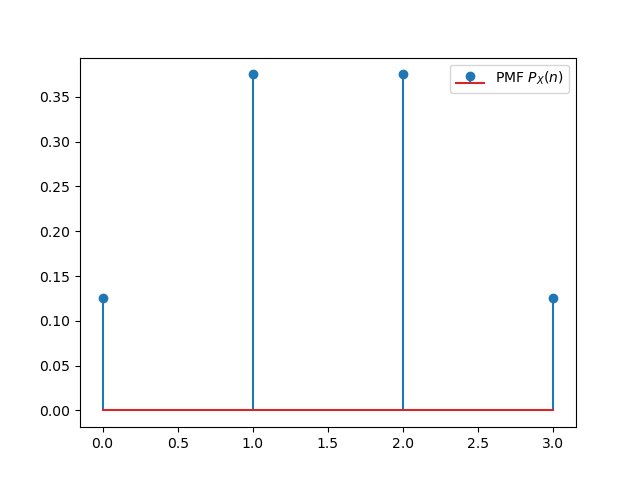
\includegraphics[width=1\columnwidth]{figs/pmf1.png}
          \label{stemplot}
        \end{figure}
      \end{frame}
      \begin{frame}[fragile]
        \frametitle{Graph}
        \begin{figure}[h!]
          \centering
          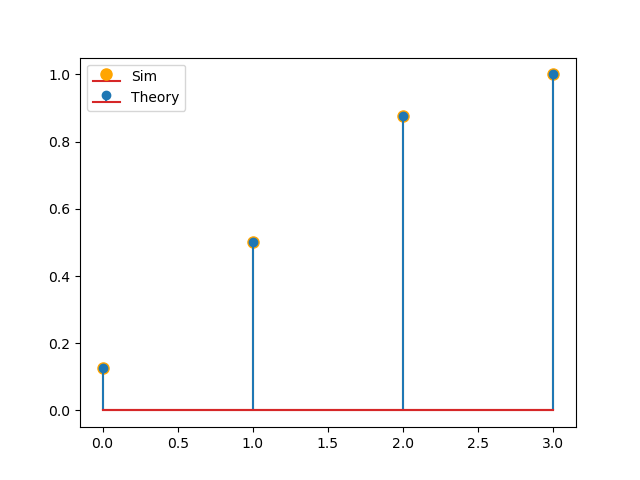
\includegraphics[width=1\columnwidth]{figs/cdf.png}
          \label{stemplot}
        \end{figure}
      \end{frame}

      \subsection{Interesting Fact}
      \begin{frame}
        We notice something interesting about PMF plots for different values of $m$. We see that it appears to converge Gaussian Distribution curve. One more interesting fact is that area under the Gaussian Distribution Curve is $1$. This further supports the fact that PMF converges to Gaussian Distribution Curve, as sum of all the probabilites $\brak{\sum p_X\brak{n} = 1}$ is $1$.  As $m \rightarrow \infty$ the PMF plot onverges to the Gaussian Distribution curve. We can visually verify this, \newline

        Below are the PMF graphs for $m = 10, 25, 500, 100$ respectively      
      \end{frame}
      \begin{frame}[fragile]
        \frametitle{Graph}
        \begin{figure}[h!]
          \centering
          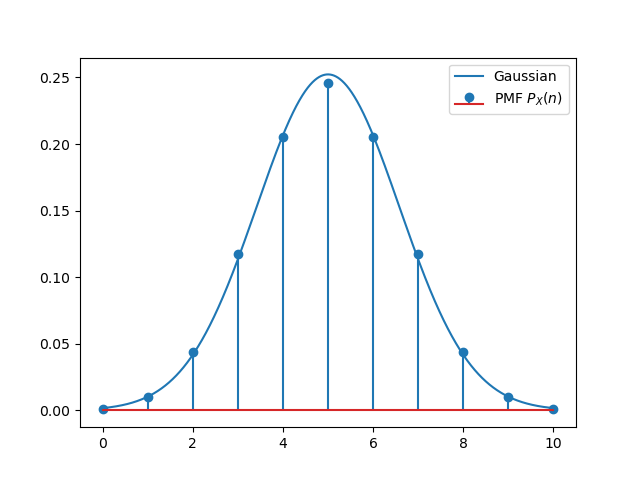
\includegraphics[width=1\columnwidth]{figs/pmf2.png}
          \label{stemplot}
        \end{figure}
      \end{frame}
      \begin{frame}[fragile]
        \frametitle{Graph}
        \begin{figure}[h!]
          \centering
          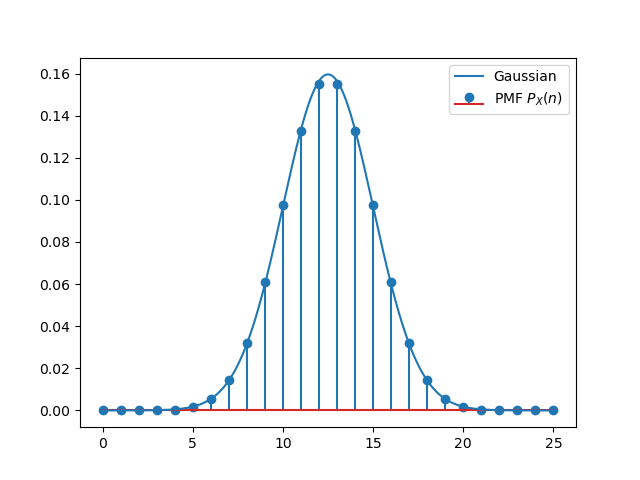
\includegraphics[width=1\columnwidth]{figs/pmf3.png}
          \label{stemplot}
        \end{figure}
      \end{frame}
      \begin{frame}[fragile]
        \frametitle{Graph}
        \begin{figure}[h!]
          \centering
          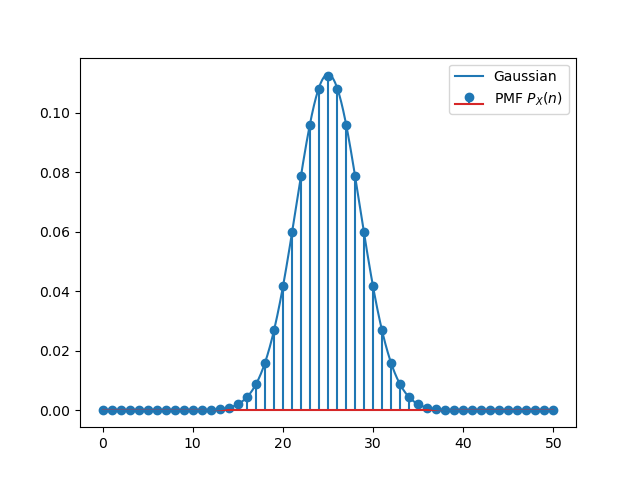
\includegraphics[width=1\columnwidth]{figs/pmf4.png}
          \label{stemplot}
        \end{figure}
      \end{frame}
      \begin{frame}[fragile]
        \frametitle{Graph}
        \begin{figure}[h!]
          \centering
          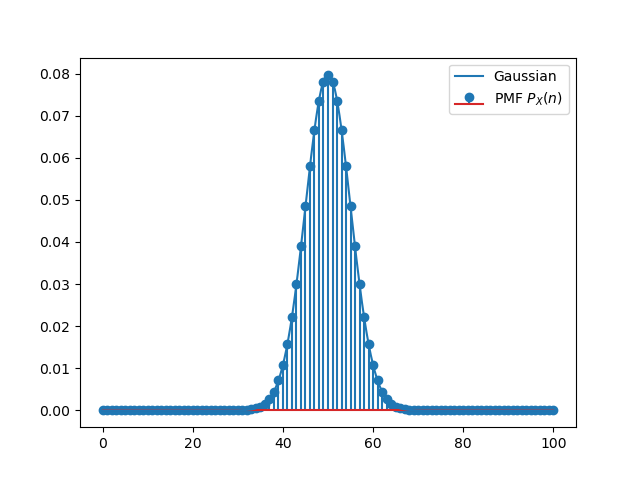
\includegraphics[width=1\columnwidth]{figs/pmf5.png}
          \label{stemplot}
        \end{figure}
      \end{frame}

    \end{document}
